%
% File emnlp2016.tex
%

\documentclass[11pt,letterpaper]{article}
\usepackage{emnlp2016}
\usepackage{times}
\usepackage{latexsym}
\usepackage{graphicx}
\graphicspath{ {images/} }

% Uncomment this line for the final submission:
%\emnlpfinalcopy

%  Enter the EMNLP Paper ID here:
\def\emnlppaperid{***}

% To expand the titlebox for more authors, uncomment
% below and set accordingly.
% \addtolength\titlebox{.5in}    

\newcommand\BibTeX{B{\sc ib}\TeX}


\title{Instructions for EMNLP 2016 Proceedings\Thanks{This
    document has been adapted from the instructions for earlier ACL
    and NAACL proceedings.}}

% Author information can be set in various styles:
% For several authors from the same institution:
% \author{Author 1 \and ... \and Author n \\
%         Address line \\ ... \\ Address line}
% if the names do not fit well on one line use
%         Author 1 \\ {\bf Author 2} \\ ... \\ {\bf Author n} \\
% For authors from different institutions:
% \author{Author 1 \\ Address line \\  ... \\ Address line
%         \And  ... \And
%         Author n \\ Address line \\ ... \\ Address line}
% To start a seperate ``row'' of authors use \AND, as in
% \author{Author 1 \\ Address line \\  ... \\ Address line
%         \AND
%         Author 2 \\ Address line \\ ... \\ Address line \And
%         Author 3 \\ Address line \\ ... \\ Address line}
% If the title and author information does not fit in the area allocated,
% place \setlength\titlebox{<new height>} right after
% at the top, where <new height> can be something larger than 2.25in
\author{Siddharth Patwardhan \and Daniele Pighin\\
  {\tt publication@emnlp2016.net}}

\date{}

\begin{document}

\maketitle

\begin{abstract}
  While there are gaps in our understanding of how the brain works to produce speech, existing research has shown promise that brain activity is discriminative enough for speech recognition. This study works towards multimodal speech recognition using signals from all modalities, including brain activity data through EEG, to better understand the role of each modality in speech production. We present trained models that incorporate audio, visual, and EEG information to perform phonetic-based speech recognition. We evaluate these models on phoneme classification tasks, showing separate results for speaker-dependent cases and speaker-independent cases. Classification rates indicate there are some discriminative features in visual and EEG signals but more data, further preprocessing, and more complex models may be required to effectively extract these features for speech recognition tasks.
\end{abstract}


\section{Introduction}

With the increase in computer processing speeds, there is a rising interest in convenient and accessible solutions for human-computer interaction and brain-computer interfaces. It comes as no surprise that such a solution would use speech, the most convenient form of communication for human society, as a primary means of interaction. Automatic speech recognition (ASR) has historically both relied on and driven machine learning techniques. Currently, special cases of Dynamic Bayes Networks (DBN) are popularly used for ASR models. With the advent of less invasive visual recognition technology to detect kinematic features, research has increased performance by including bimodal audio-visual observations in models to train ASR systems [1]. Although these models are implemented in many popular software solutions for the average consumer, further challenges arise when models have to account for speech disorders related to the physical production of speech. Classification boundaries for phonological categories or vocal tract movements become less obvious and recognition performance drops.

This research modeled facial tracking, audio, and EEG observations using machine learning models to relate the three modalities to each other during actual speech production, going beyond the bimodal audio-visual ASR systems. Necessary data for all three modalities previously existed and was originally used for binary classification of phonological categories. The KARAONE data set contains all three modalities at various states (silent speech state, stimulus state, speech production state) which made it highly suitable for comparing multimodal relationships without bias. Initially, relevant features from audio-visual as well as the continuous EEG recordings were extracted. Afterwards, various model architectures were experimented with to formulate and validate a model that best fits the KARA ONE dataset [2]. The models were then investigated on their performance in terms of their classification rates. The models helped in exploring multimodal relationships that can make meaningful contributions to various aspects of ASR.  The study was a step towards a better understanding of relationships between the relevant modalities and to provide additional support for ASR systems related to silent speech recognition, and brain-computer interfaces.

\section{Literature Review}

\subsection{Dynamic Bayesian Networks}
In the early 1990s, Paul Dagum developed the concept of Dynamic Bayes Networks [3] (DBNs) – calling them Dynamic Network Models – which can be seen as generalizing some of the more simple models for sequential data analysis like Hidden Markov Models (HMMs) [4]. DBNs are a form of traditional Bayesian probabilistic graphical models that represent conditional dependencies between random variables by using directed acyclic graphs. Various algorithms can use these models for supervised learning and inference by supplying them with evidence and historical data. DBNs, today, are applied to a variety of applications including the primary interest of this paper, multi-modal speech recognition [4]. Generally, for speech recognition, the sequential data comes in the form of temporal (time-series) data and subsequent models will therefore attempt to capture the forward moving linearity of time. Firstly, using just a static network, we can capture contemporaneous dependencies between variables, and then expand it into a dynamic network which will model these dependencies across time (Figure 2.1) [3]. The static network can be considered as a single time-slice in a DBN, which then links a time-slice to the next using directed (since we are dealing with temporal sequence data) arcs between them [5]. In this sense, DBN becomes an acyclic graph with edges representing dependencies between the vertices or variables [4]. It is important to note that the static network graph structure for each time slice does not change over time [5], as Dagum’s motivation for DBNs was simply to forecast future values of variables given the structure of the static network [3].

\begin{figure}[ht]
\centering
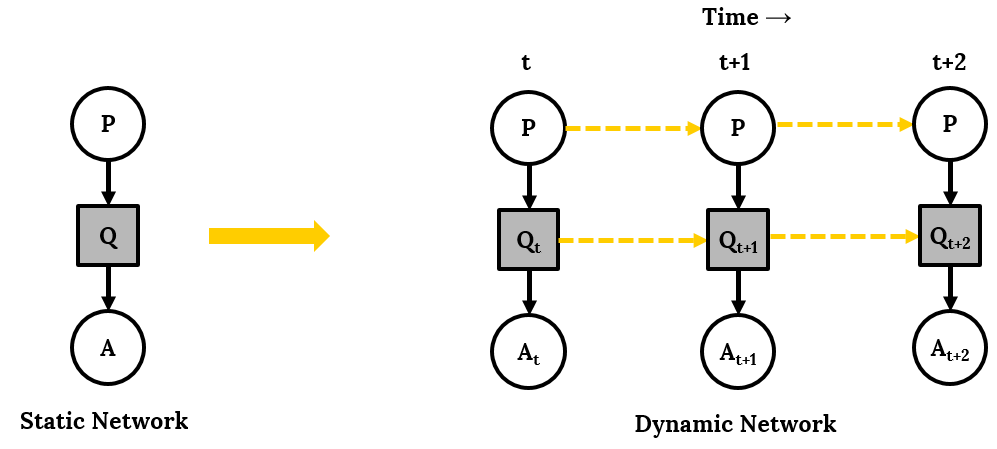
\includegraphics[scale=0.25]{dbn_description}
\caption{DBN Overview}
\end{figure}

To better understand the advantages and disadvantages of DBNs, we can start by observing HMMs, a specific case of DBNs. A simple variant – there are more complicated versions which still fall under the DBN generalization – of an HMM represents the hidden state of the world using a single discrete random variable, $X_t$, which can take on various values [5]. The hidden state can be considered to generate an observation (represented by an arc leading from the former to the latter) which is modeled by another random variable, $Y_t$ . The directed relationship between $X_t$ and $Y_t$ can be considered a single time slice or the static network. Placing a directed arc between the hidden states of one time slice to the next (e.g. $X_1$ to $X_2$) will form a dynamic network [3]. Figure 2.2 depicts a simple HMM as described above. Similarly, we can form a graph with more than one variable to represent the hidden state and more than one variable to represent the observed state, generalizing the HMM to a DBN [5].To better understand the advantages and disadvantages of DBNs, we can start by observing HMMs, a specific case of DBNs. A simple variant – there are more complicated versions which still fall under the DBN generalization – of an HMM represents the hidden state of the world using a single discrete random variable, $X_t$, which can take on various values [5]. The hidden state can be considered to generate an observation (represented by an arc leading from the former to the latter) which is modeled by another random variable, $Y_t$ . The directed relationship between $X_t$ and $Y_t$ can be considered a single time slice or the static network. Placing a directed arc between the hidden states of one time slice to the next (e.g. $X_1$ to $X_2$) will form a dynamic network [3]. Figure 2.2 depicts a simple HMM as described above. Similarly, we can form a graph with more than one variable to represent the hidden state and more than one variable to represent the observed state, generalizing the HMM to a DBN [5].

\section{Data}

The database – KARAONE [2] – used for this study is available to the public and contains all three modalities that are of interest to this paper – audio-visual data as well as complimentary EEG data. All three modalities were collected during a stimulus state – prompt text appeared on screen –, a silent/imagine speech state – participant imagined speaking the prompt without actual production –, and a speaking stage – where the participant spoke the prompt out loud [2]. Data is available for 14 participants who were prompted 12 times for each of the 11 prompts (a total of 132 trial for each participant), which were a mix of phonemic and isolated word prompts. The study, concerned with end-to-end learning of phonetic-based ASR, dealt with only the 7 phonemic prompts (/uw/, /tiy/, /iy/, /m/, /n/, /piy/, /diy/). 

The KARAONE [2] database has certain advantages that makes it suitable for our purposes. Since we are primarily concerned with finding multi-modal relationships that can benefit speech recognition or brain-computer interfaces, the methods through which data was collected are advantageous. Visual data is collected using relatively simple means through a consumer product [2] which makes it feasible to use for modeling practical conditions. Furthermore, accessing language centers directly can be invasive to achieve ideal and high SNRs [15, 2] but EEG recordings are a more accessible and applicable solution [15, 2], and by definition, non-invasive. Once again, for our purposes, working with data that is more accessible is advantageous since general brain-computer interfaces or ASR systems will not have access to more intrusive methods, even if they can provide less noisy data. Furthermore, the KARAONE database contains data from both silent speech and spoken speech states [2] for the same prompts which is ideal for our purpose of determining multi-modal relationships. Access to neural activity relatively uncontaminated by physiological artifacts [14, 15] allows us to make unbiased comparisons with audio-visual modalities. Lastly, since the database contains data from multiple speakers, it allows this study to explore speaker-independent multi-modal speech recognition as well.  

\subsection{Audio Data}
Audio Data was available in the form of .wav files, sampled at 16 KHz and each trail separated into a unique file. Each of these audio segments were converted into 42 dimension vectors of Mel-Frequency Cepstral Coefficients (MFCC) across time using VOICEBOX [19], a speech processing toolbox for MATLAB under a GNU Public license.

\subsection{Visual Data}
The visual data in the database used a Microsoft Kinect camera [20] to record the participants during trials. For each frame of the captured video, 6 Animation Units (AUs) – ranging between -1 to +1 – were extracted corresponding to Figure 3.1. AU values were obtained from .AU files within the database and could be up-sampled such that both the Visual data and the MFCC data had the same total number of time slices for each trial. At each time-slice, the visual data consisted of a 6-dimension vector.

\subsection{EEG Data}
EEG data was available in the form of a .cnt file in the database [2], from which continuous 64-dimension (one for each electrode) data was extracted using EEGLAB, an open source MATLAB environment for electrophysiological signal processing [21].  Only 10 of the 64 channels were used as training data as they proved to be the most discriminative features from previous research [2]. The electrode positioning followed the 10-20 system, see Figure 2.7. Note that we are working with EEG data during the imagined/silence speech state since during other stages, the recording contain a large amount of artifacts (e.g. from screen, muscle movement, etc.).

\section{Methodology}
This study designed and trained models incorporating information from all relevant modalities. Using 9-fold cross validation for speaker dependent speech recognition models and 10-fold cross validation for speaker independent speech recognition models, the models were evaluated by their classification rates. The design, creation, and training of the models is discussed in the following sub sections. 

\subsection{DBN Design}
Dynamic Bayes Networks were designed in MATLAB for this study, using Kevin Murphy’s open source Bayes Net Toolbox (BNT) [22]. BNT supports not only the design of DBNs but also supports many inference algorithms and methods (Figure 2.3). Two separate DBNs were designed, one for EEG modeling, the other incorporating audio-visual modes. Since the EEG data being used is during the ‘silent-speech’ state, it is not synchronous with the audio-visual data which is for the ‘speech-production’ state and a separate DBN for the EEG mode was necessary.

Our EEG DBN, depicted in Figure 4.1, is defined as a GMM-HMM, where a Gaussian mixture model, with 12 multivariate Gaussians, occupies a node. Otherwise, the phoneme (P) and hidden state (Q) nodes are discrete nodes while node E contains the continuous observed EEG feature vectors at each time step. The only interdependencies across time steps is a connection between the hidden nodes.

The audio-visual DBN (Figure 4.2) models phonemes (P), visual data (V), and the hidden state (Q) with discrete nodes while node A contains continuous observed MFCC coefficients across time steps. The visual data, up-sampled to match the temporal length of our audio data, is preprocessed with K-means algorithm into clusters to convert it from continuous to discrete. As visible in Figure 4.2, the audio data is conditionally dependent on all other nodes while the visual data is only conditionally dependent on nodes P and Q. Theoretically, this models the dependency of the produced speech on the positions of certain facial features (e.g. curve of the lips). 

Final classifications were performed by taking into account the likelihood of test data being generated by a certain phoneme, for each DBN. 

\begin{figure}[h]
\centering
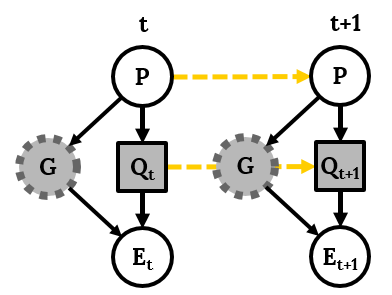
\includegraphics[scale=0.5]{dbn_design_eeg}
\caption{EEG DBN Design}
\end{figure}

\begin{figure}[h]
\centering
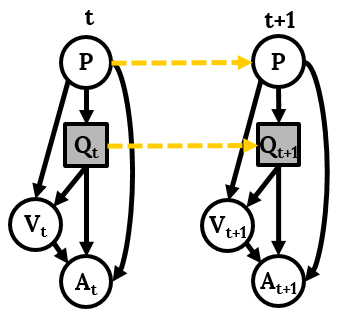
\includegraphics[scale=0.5]{dbn_design_audio}
\caption{Audio-visual DBN Design}
\end{figure}

\subsection{RNN Design}
The second approach to multi-modal speech recognition in this study involved the use of recurrent neural networks to capture temporal dependencies for each mode and integrate the modes together to train a multi-layer perceptron. Figure 4.3 illustrates the complete architecture for training our multi-modal phoneme classifier. The training data ($x_A,x_V,x_E$) – 42-dimension audio MFCCs, 6-dimension visual Kinect AU units, 10-dimension raw EEG data – for each RNN consisted of the data for each mode labeled with the respective phoneme. The hidden units of the RNNs were LSTM cells to increase memory of model. Figure 4.4 shows the final parameters used for training after various trials and error to determine those resulting in best performance. Once each separate RNN model was trained, the output of the hidden layer in the last time step $(h_A^((T_A ) ),h_V^((T_V ) ),h_E^((T_E ) ))$ for each training case was taken as training data for a multi-layer perceptron, consisting of sigmoid activations. These architectures were designed and coded using Theano in python.

\begin{figure}[h]
\centering
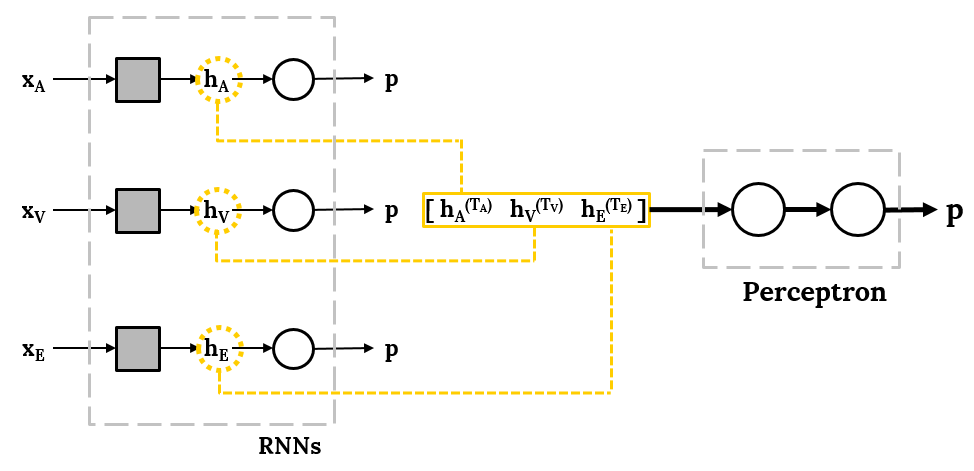
\includegraphics[scale=0.25]{rnn_design}
\caption{RNN Architecture}
\end{figure}


\section{Results}
For this study, there are two aspects to highlight in terms of results. Firstly, we will present the performance of the trained ASR systems in terms of their classification rates. Secondly, we can compare and contrast the contributions of each mode to overall performance. The performance measure for these models is generally their error rates on validation data and we specifically concern ourselves with precision, recall, and F1 score.

Precision, for each class, is the number of true positives over the number of true positives plus the number of false positives:

$P=T_p/(T_p+F_p )$

Recall, for each class, is the number of true positives over the number of true positives plus the number of false negatives:

$R=T_p/(T_p+F_n )$

Precision and Recall are also related to the F1 score, which is defined as the harmonic mean of precision and recall:

$F1=2 (P*R)/(P+R)$

Tables go here:


\section{Discussions}
Comparing results across models and modes, it is clear that phoneme classification for the KARAONE dataset was better suited to RNNs – resulting in up to 87\% average precision for the speaker independent case – rather than the more traditional DBNs. In terms of modes, as expected, audio and visual data was able to discriminate between the phonemes more effectively than EEG data. However, it is important to note that audio data – and even visual data for DBNs – was preprocessed with known methods to increase performance. This was not the case with EEG data, which was inputted raw into machine learning models only to gain more understanding of its discriminative features. It was found that more EEG data was needed to effectively train a model. 

Further work is required to determine the potential of EEG data in brain-computer interfaces. Currently, only simplistic models that were effective for the audio mode were used with the EEG data but it seems EEG data may require a higher level of complexity. Deeper RNN models, bi-directional RNNs, or RNN and HMM hybrids may be a good next step in that direction. Furthermore, since little is known about the workings of the brain, we may need to approach EEG data differently than we approach other modes. One such approach could be the addition of attention mechanisms in RNNs. An instance of such models are Recurrent Neural Networks with Visual Attention [23] which can be trained using reinforcement learning methods and adaptively focus on and process certain regions from the input data. Since we do not have knowledge about which regions and sequences of EEG data are the most discriminative, this approach may successfully learn the patterns that basic models are missing. Nevertheless, given the promising existing research around the EEG mode, experimentation to extract the discriminative features from EEG data is a natural direction for future work. 


\section*{Acknowledgments}

Do not number the acknowledgment section.

\bibliography{emnlp2016}
\bibliographystyle{emnlp2016}

\end{document}
